\scanpage{65}
$M_n\subset I^n\qquad n\in\mathbb N\qquad(I=[-1,+1])$

$M_n$ stable par int. et réunions finies.

$M_*$ stables par images directes et inverses d'appl. simpliciales.

$M_0$ contient \deleted{\unsure{tous pts de coordonnées entières|tous points de coordonnées entières}} $\{0\}$ et $\{1\}$

\deleted{$\unsure{M_{n+1}}$}
$\left[\left\{\begin{array}{l}
I\text{ est }\mathcal M\text{-injectif (se traduit en termes de }M_*\text{)}\\
\text{Tout }\deleted{\text{élément objet de}}\ \inserted{M_n}\text{ est de la forme }
f^{-1}(0)=\displaystyle\bigcap_{1\leq i\leq p}f_i^{-1}(0)\\
f:I^n-I^p\text{ ``permis'')}
\end{array}\right.\right]$
\margin{$\Longrightarrow$}

a) $M_{\deleted{\unsure{*}}}$ contient les simplexes types et \deleted{leurs applications} \inserted{une} application lin. d'un simplexe type dans $I$ est un $\mathcal M$-morphisme ssi \deleted{\unsure{ses applications}} ses valeurs aux sommets le sont.

b) Pour tout \deleted{un} ``schéma simplicial'' fini $\Sigma$, sa réalisation
\deleted{Soit $\mathcal M^0$ la catégorie des \unsure{espaces cpts|espaces épts} lin. par morceaux.}
géométrique $\widetilde\Sigma$ admet une $\mathcal M$-structure admissible (définie par une $\unsure{\varinjlim|\uline{\lim}}$ finie dans $\mathcal M$), et \inserted{c)} tout objet de $\mathcal M$ [i.e. \deleted{\unsure{de}} élément d'un $M_n$] admet une telle ``\uline{triangulation}''.
Pour tout couple $Y\subset X$ dans $\mathcal M$ (OPS $Y,X\in M_n$, $Y\subset X$), \deleted{\unsure{si}} tt \deleted{\unsure{de}} $\mathcal M$-\uline{triangulation} de $Y$ est induite par une $\mathcal M$-\uline{triangulation} de $X$.

\figure{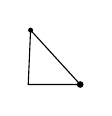
\begin{tikzpicture}[scale=.6]
\draw (0,0)--(.05,1.15)--(1.1,0)--cycle;
\fill (.05,1.15) circle (1.5pt); \fill (1.1,0) circle (2pt);
\end{tikzpicture}}
\[
\left\{(x_0-x_n;y)\ \middle|\ 
\left\{\begin{array}{l}
x_i\geq0\qquad\sum x_i=1\\
y\unsure{-}\displaystyle\sum_{0\leq i\leq n}a_i x_i=0
\end{array}\right.\right\}\in M_{n+2}
\]
si les $\{a_i\}\in M_1$

\margin{UNIVERSITE DES SCIENCES ET TECHNIQUES\\
DU LANGUEDOC\\
---\\
INSTITUT DE MATHEMATIQUES\\
Place Eugène Bataillon\\
34060 MONTPELLIER CEDEX\\
---\\
Montpellier, le}

\margin{66}
